\documentclass[12pt]{article}\usepackage[]{graphicx}\usepackage[]{color}
%% maxwidth is the original width if it is less than linewidth
%% otherwise use linewidth (to make sure the graphics do not exceed the margin)
\makeatletter
\def\maxwidth{ %
  \ifdim\Gin@nat@width>\linewidth
    \linewidth
  \else
    \Gin@nat@width
  \fi
}
\makeatother

\definecolor{fgcolor}{rgb}{0.345, 0.345, 0.345}
\newcommand{\hlnum}[1]{\textcolor[rgb]{0.686,0.059,0.569}{#1}}%
\newcommand{\hlstr}[1]{\textcolor[rgb]{0.192,0.494,0.8}{#1}}%
\newcommand{\hlcom}[1]{\textcolor[rgb]{0.678,0.584,0.686}{\textit{#1}}}%
\newcommand{\hlopt}[1]{\textcolor[rgb]{0,0,0}{#1}}%
\newcommand{\hlstd}[1]{\textcolor[rgb]{0.345,0.345,0.345}{#1}}%
\newcommand{\hlkwa}[1]{\textcolor[rgb]{0.161,0.373,0.58}{\textbf{#1}}}%
\newcommand{\hlkwb}[1]{\textcolor[rgb]{0.69,0.353,0.396}{#1}}%
\newcommand{\hlkwc}[1]{\textcolor[rgb]{0.333,0.667,0.333}{#1}}%
\newcommand{\hlkwd}[1]{\textcolor[rgb]{0.737,0.353,0.396}{\textbf{#1}}}%
\let\hlipl\hlkwb

\usepackage{framed}
\makeatletter
\newenvironment{kframe}{%
 \def\at@end@of@kframe{}%
 \ifinner\ifhmode%
  \def\at@end@of@kframe{\end{minipage}}%
  \begin{minipage}{\columnwidth}%
 \fi\fi%
 \def\FrameCommand##1{\hskip\@totalleftmargin \hskip-\fboxsep
 \colorbox{shadecolor}{##1}\hskip-\fboxsep
     % There is no \\@totalrightmargin, so:
     \hskip-\linewidth \hskip-\@totalleftmargin \hskip\columnwidth}%
 \MakeFramed {\advance\hsize-\width
   \@totalleftmargin\z@ \linewidth\hsize
   \@setminipage}}%
 {\par\unskip\endMakeFramed%
 \at@end@of@kframe}
\makeatother

\definecolor{shadecolor}{rgb}{.97, .97, .97}
\definecolor{messagecolor}{rgb}{0, 0, 0}
\definecolor{warningcolor}{rgb}{1, 0, 1}
\definecolor{errorcolor}{rgb}{1, 0, 0}
\newenvironment{knitrout}{}{} % an empty environment to be redefined in TeX

\usepackage{alltt}
 
\usepackage[margin=1in]{geometry}
\usepackage{amsmath,amsthm,amssymb, mathtools}
\usepackage[T1]{fontenc}
\usepackage{lmodern}
 
\newcommand{\N}{\mathbb{N}}
\newcommand{\R}{\mathbb{R}}
\newcommand{\Z}{\mathbb{Z}}
\newcommand{\Q}{\mathbb{Q}}
 
\newenvironment{theorem}[2][Theorem]{\begin{trivlist}
\item[\hskip \labelsep {\bfseries #1}\hskip \labelsep {\bfseries #2.}]}{\end{trivlist}}
\newenvironment{lemma}[2][Lemma]{\begin{trivlist}
\item[\hskip \labelsep {\bfseries #1}\hskip \labelsep {\bfseries #2.}]}{\end{trivlist}}
\newenvironment{exercise}[2][Exercise]{\begin{trivlist}
\item[\hskip \labelsep {\bfseries #1}\hskip \labelsep {\bfseries #2.}]}{\end{trivlist}}
\newenvironment{problem}[2][Problem]{\begin{trivlist}
\item[\hskip \labelsep {\bfseries #1}\hskip \labelsep {\bfseries #2.}]}{\end{trivlist}}
\newenvironment{question}[2][Question]{\begin{trivlist}
\item[\hskip \labelsep {\bfseries #1}\hskip \labelsep {\bfseries #2.}]}{\end{trivlist}}
\newenvironment{corollary}[2][Corollary]{\begin{trivlist}
\item[\hskip \labelsep {\bfseries #1}\hskip \labelsep {\bfseries #2.}]}{\end{trivlist}}
\newcommand{\textfrac}[2]{\dfrac{\text{#1}}{\text{#2}}}
\IfFileExists{upquote.sty}{\usepackage{upquote}}{}
\begin{document}

\title{Statistical Rethinking: Chapter 3 - Sampling the Imaginary}

\author{Chris Hayduk}
\date{\today}

\maketitle




\section{Easy}

These problems use the samples from the posterior distribution for the globe tossing example. This code will give you a specific set of samples, so that you can check your answers exactly.

\begin{knitrout}
\definecolor{shadecolor}{rgb}{0.969, 0.969, 0.969}\color{fgcolor}\begin{kframe}
\begin{alltt}
\hlstd{p_grid} \hlkwb{<-} \hlkwd{seq}\hlstd{(}\hlkwc{from} \hlstd{=} \hlnum{0}\hlstd{,} \hlkwc{to} \hlstd{=} \hlnum{1}\hlstd{,} \hlkwc{length.out} \hlstd{=} \hlnum{1000}\hlstd{)}
\hlstd{prior} \hlkwb{<-} \hlkwd{rep}\hlstd{(}\hlnum{1}\hlstd{,} \hlnum{1000}\hlstd{)}
\hlstd{likelihood} \hlkwb{<-} \hlkwd{dbinom}\hlstd{(}\hlnum{6}\hlstd{,} \hlkwc{size} \hlstd{=} \hlnum{9}\hlstd{,} \hlkwc{prob} \hlstd{= p_grid)}
\hlstd{posterior} \hlkwb{<-} \hlstd{likelihood} \hlopt{*} \hlstd{prior}
\hlstd{posterior} \hlkwb{<-} \hlstd{posterior} \hlopt{/} \hlkwd{sum}\hlstd{(posterior)}
\hlkwd{set.seed}\hlstd{(}\hlnum{100}\hlstd{)}
\hlstd{samples} \hlkwb{<-} \hlkwd{sample}\hlstd{(p_grid,} \hlkwc{prob} \hlstd{= posterior,} \hlkwc{size} \hlstd{=} \hlnum{1e4}\hlstd{,} \hlkwc{replace} \hlstd{=} \hlnum{TRUE}\hlstd{)}
\end{alltt}
\end{kframe}
\end{knitrout}

Use the values in \textit{samples} to answer the questions that follow.

\begin{problem}{3E1}
\text{}\\
How much posterior probability lies below p = 0.2?
\end{problem}

\begin{knitrout}
\definecolor{shadecolor}{rgb}{0.969, 0.969, 0.969}\color{fgcolor}\begin{kframe}
\begin{alltt}
\hlkwd{sum}\hlstd{(samples} \hlopt{<} \hlnum{0.2}\hlstd{)} \hlopt{/} \hlnum{1e4}
\end{alltt}
\begin{verbatim}
## [1] 5e-04
\end{verbatim}
\end{kframe}
\end{knitrout}

\begin{problem}{3E2}
\text{}\\
How much posterior probability lies above p = 0.8?
\end{problem}

\begin{knitrout}
\definecolor{shadecolor}{rgb}{0.969, 0.969, 0.969}\color{fgcolor}\begin{kframe}
\begin{alltt}
\hlkwd{sum}\hlstd{(samples} \hlopt{>} \hlnum{0.8}\hlstd{)} \hlopt{/} \hlnum{1e4}
\end{alltt}
\begin{verbatim}
## [1] 0.1117
\end{verbatim}
\end{kframe}
\end{knitrout}

\begin{problem}{3E3}
\text{}\\
How much posterior probability lies between p = 0.2 and p = 0.8?
\end{problem}

\begin{knitrout}
\definecolor{shadecolor}{rgb}{0.969, 0.969, 0.969}\color{fgcolor}\begin{kframe}
\begin{alltt}
\hlkwd{sum}\hlstd{(samples} \hlopt{>} \hlnum{0.2} \hlopt{&} \hlstd{samples} \hlopt{<} \hlnum{0.8}\hlstd{)} \hlopt{/} \hlnum{1e4}
\end{alltt}
\begin{verbatim}
## [1] 0.8878
\end{verbatim}
\end{kframe}
\end{knitrout}

\begin{problem}{3E4}
\text{}\\
20\% of the posterior probability lies below which value of p?
\end{problem}

\begin{knitrout}
\definecolor{shadecolor}{rgb}{0.969, 0.969, 0.969}\color{fgcolor}\begin{kframe}
\begin{alltt}
\hlkwd{quantile}\hlstd{(samples,} \hlnum{0.2}\hlstd{)}
\end{alltt}
\begin{verbatim}
##       20% 
## 0.5195195
\end{verbatim}
\end{kframe}
\end{knitrout}

\begin{problem}{3E5}
\text{}\\
20\% of the posterior probability lies above which value of p?
\end{problem}

\begin{knitrout}
\definecolor{shadecolor}{rgb}{0.969, 0.969, 0.969}\color{fgcolor}\begin{kframe}
\begin{alltt}
\hlkwd{quantile}\hlstd{(samples,} \hlnum{0.8}\hlstd{)}
\end{alltt}
\begin{verbatim}
##       80% 
## 0.7567568
\end{verbatim}
\end{kframe}
\end{knitrout}

\begin{problem}{3E6}
\text{}\\
Which values of p contain the narrowest interval equal to 66\% of the posterior probability?
\end{problem}

\begin{knitrout}
\definecolor{shadecolor}{rgb}{0.969, 0.969, 0.969}\color{fgcolor}\begin{kframe}
\begin{alltt}
\hlkwd{HPDI}\hlstd{(samples,} \hlkwc{prob} \hlstd{=} \hlnum{0.66}\hlstd{)}
\end{alltt}
\begin{verbatim}
##     |0.66     0.66| 
## 0.5205205 0.7847848
\end{verbatim}
\end{kframe}
\end{knitrout}

\begin{problem}{3E7}
\text{}\\
Which values of p contain 66\% of the posterior probability, assuming equal posterior probability both below and above the interval?
\end{problem}

\begin{knitrout}
\definecolor{shadecolor}{rgb}{0.969, 0.969, 0.969}\color{fgcolor}\begin{kframe}
\begin{alltt}
\hlkwd{PI}\hlstd{(samples,} \hlkwc{prob} \hlstd{=} \hlnum{0.66}\hlstd{)}
\end{alltt}
\begin{verbatim}
##       17%       83% 
## 0.5005005 0.7687688
\end{verbatim}
\end{kframe}
\end{knitrout}

\section{Medium}

\begin{problem}{3M1}
\text{}\\
Suppose the globe tossing data had turned out to be 8 water in 15 tosses. Construct the posterior distribution, using grid approximation. Use the same flat prior as before.
\end{problem}

\begin{knitrout}
\definecolor{shadecolor}{rgb}{0.969, 0.969, 0.969}\color{fgcolor}\begin{kframe}
\begin{alltt}
\hlstd{p_grid} \hlkwb{<-} \hlkwd{seq}\hlstd{(}\hlkwc{from} \hlstd{=} \hlnum{0}\hlstd{,} \hlkwc{to} \hlstd{=} \hlnum{1}\hlstd{,} \hlkwc{length.out} \hlstd{=} \hlnum{1000}\hlstd{)}
\hlstd{prior} \hlkwb{<-} \hlkwd{rep}\hlstd{(}\hlnum{1}\hlstd{,} \hlnum{1000}\hlstd{)}
\hlstd{likelihood} \hlkwb{<-} \hlkwd{dbinom}\hlstd{(}\hlnum{8}\hlstd{,} \hlkwc{size} \hlstd{=} \hlnum{15}\hlstd{,} \hlkwc{prob} \hlstd{= p_grid)}
\hlstd{posterior} \hlkwb{<-} \hlstd{likelihood}\hlopt{*}\hlstd{prior}
\hlstd{posterior} \hlkwb{<-} \hlstd{posterior} \hlopt{/} \hlkwd{sum}\hlstd{(posterior)}
\end{alltt}
\end{kframe}
\end{knitrout}

\begin{problem}{3M2}
\text{}\\
Draw 10,000 samples from the grid approximation from above. Then use the samples to calculate the 90\% HDPI for p.
\end{problem}

\begin{knitrout}
\definecolor{shadecolor}{rgb}{0.969, 0.969, 0.969}\color{fgcolor}\begin{kframe}
\begin{alltt}
\hlstd{samples} \hlkwb{<-} \hlkwd{sample}\hlstd{(p_grid,} \hlkwc{prob} \hlstd{= posterior,} \hlkwc{size} \hlstd{=} \hlnum{1e4}\hlstd{,} \hlkwc{replace} \hlstd{=} \hlnum{TRUE}\hlstd{)}

\hlkwd{HPDI}\hlstd{(samples,} \hlkwc{prob} \hlstd{=} \hlnum{0.9}\hlstd{)}
\end{alltt}
\begin{verbatim}
##      |0.9      0.9| 
## 0.3383383 0.7317317
\end{verbatim}
\end{kframe}
\end{knitrout}

\begin{problem}{3M3}
\text{}\\
Construct a posterior predictive check for this model and data. This means simulate the distribution of samples, averaging over the posterior uncertainty in p. What is the probability of observing 8 water in 15 tosses?
\end{problem}

\begin{knitrout}
\definecolor{shadecolor}{rgb}{0.969, 0.969, 0.969}\color{fgcolor}\begin{kframe}
\begin{alltt}
\hlstd{w} \hlkwb{<-} \hlkwd{rbinom}\hlstd{(}\hlnum{1e4}\hlstd{,} \hlkwc{size} \hlstd{=} \hlnum{15}\hlstd{,} \hlkwc{prob} \hlstd{= samples)}

\hlkwd{sum}\hlstd{(w[}\hlkwc{w} \hlstd{=} \hlnum{8}\hlstd{])} \hlopt{/} \hlnum{1e4}
\end{alltt}
\begin{verbatim}
## [1] 0.0012
\end{verbatim}
\end{kframe}
\end{knitrout}

\begin{problem}{3M4}
\text{}\\
Using the posterior distribution constructed from the nw (8/15) data, now calculate the probability of observing 6 water in 9 tosses.
\end{problem}

\begin{knitrout}
\definecolor{shadecolor}{rgb}{0.969, 0.969, 0.969}\color{fgcolor}\begin{kframe}
\begin{alltt}
\hlstd{w} \hlkwb{<-} \hlkwd{rbinom}\hlstd{(}\hlnum{1e4}\hlstd{,} \hlkwc{size} \hlstd{=} \hlnum{9}\hlstd{,} \hlkwc{prob} \hlstd{= samples)}

\hlkwd{sum}\hlstd{(w[}\hlkwc{w} \hlstd{=} \hlnum{6}\hlstd{])} \hlopt{/} \hlnum{1e4}
\end{alltt}
\begin{verbatim}
## [1] 1e-04
\end{verbatim}
\end{kframe}
\end{knitrout}

\begin{problem}{3M5}
\text{}\\
Start over at 3M1, but now use a prior that is zero below p = 0.5 and a constant above p = 0.5. This corresponds to prior information that a majority of the Earth's surface is water. Repeat each problem above and compare the inferences. What difference does the better prior make? If it helps, compare inferences (using both priors) to the true value p = 0.7.
\end{problem}

\begin{knitrout}
\definecolor{shadecolor}{rgb}{0.969, 0.969, 0.969}\color{fgcolor}\begin{kframe}
\begin{alltt}
\hlcom{#Re-doing 3M1}
\hlstd{p_grid} \hlkwb{<-} \hlkwd{seq}\hlstd{(}\hlkwc{from} \hlstd{=} \hlnum{0}\hlstd{,} \hlkwc{to} \hlstd{=} \hlnum{1}\hlstd{,} \hlkwc{length.out} \hlstd{=} \hlnum{1000}\hlstd{)}
\hlstd{prior} \hlkwb{<-} \hlkwd{ifelse}\hlstd{(p_grid} \hlopt{<} \hlnum{0.5}\hlstd{,} \hlnum{0}\hlstd{,} \hlnum{1}\hlstd{)}
\hlstd{likelihood} \hlkwb{<-} \hlkwd{dbinom}\hlstd{(}\hlnum{8}\hlstd{,} \hlkwc{size} \hlstd{=} \hlnum{15}\hlstd{,} \hlkwc{prob} \hlstd{= p_grid)}
\hlstd{posterior} \hlkwb{<-} \hlstd{likelihood}\hlopt{*}\hlstd{prior}
\hlstd{posterior} \hlkwb{<-} \hlstd{posterior} \hlopt{/} \hlkwd{sum}\hlstd{(posterior)}

\hlcom{#Re-doing 3M2}
\hlstd{samples} \hlkwb{<-} \hlkwd{sample}\hlstd{(p_grid,} \hlkwc{prob} \hlstd{= posterior,} \hlkwc{size} \hlstd{=} \hlnum{1e4}\hlstd{,} \hlkwc{replace} \hlstd{=} \hlnum{TRUE}\hlstd{)}

\hlkwd{HPDI}\hlstd{(samples,} \hlkwc{prob} \hlstd{=} \hlnum{0.9}\hlstd{)}
\end{alltt}
\begin{verbatim}
##      |0.9      0.9| 
## 0.5005005 0.7097097
\end{verbatim}
\begin{alltt}
\hlcom{#Re-doing 3M3}
\hlstd{w} \hlkwb{<-} \hlkwd{rbinom}\hlstd{(}\hlnum{1e4}\hlstd{,} \hlkwc{size} \hlstd{=} \hlnum{15}\hlstd{,} \hlkwc{prob} \hlstd{= samples)}

\hlkwd{sum}\hlstd{(w[}\hlkwc{w} \hlstd{=} \hlnum{8}\hlstd{])} \hlopt{/} \hlnum{1e4}
\end{alltt}
\begin{verbatim}
## [1] 6e-04
\end{verbatim}
\begin{alltt}
\hlcom{#Re-doing 3M4}
\hlstd{w} \hlkwb{<-} \hlkwd{rbinom}\hlstd{(}\hlnum{1e4}\hlstd{,} \hlkwc{size} \hlstd{=} \hlnum{9}\hlstd{,} \hlkwc{prob} \hlstd{= samples)}

\hlkwd{sum}\hlstd{(w[}\hlkwc{w} \hlstd{=} \hlnum{6}\hlstd{])} \hlopt{/} \hlnum{1e4}
\end{alltt}
\begin{verbatim}
## [1] 5e-04
\end{verbatim}
\end{kframe}
\end{knitrout}

The HPDI is now a much narrower interval.

Since we eliminated many values that are far from the true value p = 0.7 through the use of our prior, the probability of observing 8 instances of water in 15 tosses is now much lower. The expected instances of water in 15 tosses with p = 0.7 is 10.5.

The expected instances of water in 9 tosses with p = 0.7 is 6.3. Once again, since we have eliminated many p values that are far from the true value p = 0.7, our estimate of the probability of seeing 6 instances of water in 9 tosses has improved. Since it is very close to the true value of p, the probability of seeing 6 instances of water in 9 tosses has increased with the new prior.

\section{Hard}

The practice problems here all use the dataset homeworkch3 from the rethinking package. This data indiactes the gender (male = 1, female = 0) of officially reported first and second born children in 100 two-child families.

\begin{knitrout}
\definecolor{shadecolor}{rgb}{0.969, 0.969, 0.969}\color{fgcolor}\begin{kframe}
\begin{alltt}
\hlkwd{data}\hlstd{(homeworkch3)}
\end{alltt}
\end{kframe}
\end{knitrout}

Use these vectors as data. So for example to compute the total number of boys born across all of these births, you could use:

\begin{knitrout}
\definecolor{shadecolor}{rgb}{0.969, 0.969, 0.969}\color{fgcolor}\begin{kframe}
\begin{alltt}
\hlkwd{sum}\hlstd{(birth1)} \hlopt{+} \hlkwd{sum}\hlstd{(birth2)}
\end{alltt}
\begin{verbatim}
## [1] 111
\end{verbatim}
\end{kframe}
\end{knitrout}

\begin{problem}{3H1}
\text{}\\
Using grid approximation, compute the posterior distribution for the probability of a birth being a boy. Assume a uniform prior probability. Which parameter value maximizes the posterior probability?
\end{problem}

\begin{knitrout}
\definecolor{shadecolor}{rgb}{0.969, 0.969, 0.969}\color{fgcolor}\begin{kframe}
\begin{alltt}
\hlstd{p_grid} \hlkwb{<-} \hlkwd{seq}\hlstd{(}\hlkwc{from} \hlstd{=} \hlnum{0}\hlstd{,} \hlkwc{to} \hlstd{=} \hlnum{1}\hlstd{,} \hlkwc{length.out} \hlstd{=} \hlnum{1000}\hlstd{)}
\hlstd{prior} \hlkwb{<-} \hlkwd{rep}\hlstd{(}\hlnum{1}\hlstd{,} \hlnum{1000}\hlstd{)}

\hlstd{boys} \hlkwb{<-} \hlkwd{sum}\hlstd{(birth1)} \hlopt{+} \hlkwd{sum}\hlstd{(birth2)}
\hlstd{births} \hlkwb{<-} \hlkwd{length}\hlstd{(birth1)} \hlopt{+} \hlkwd{length}\hlstd{(birth2)}

\hlstd{likelihood} \hlkwb{<-} \hlkwd{dbinom}\hlstd{(boys,} \hlkwc{size} \hlstd{= births,} \hlkwc{prob} \hlstd{= p_grid)}
\hlstd{posterior} \hlkwb{<-} \hlstd{likelihood}\hlopt{*}\hlstd{prior}
\hlstd{posterior} \hlkwb{<-} \hlstd{posterior} \hlopt{/} \hlkwd{sum}\hlstd{(posterior)}

\hlstd{p_grid[}\hlkwd{which.max}\hlstd{(posterior)]}
\end{alltt}
\begin{verbatim}
## [1] 0.5545546
\end{verbatim}
\end{kframe}
\end{knitrout}

\begin{problem}{3H2}
\text{}\\
Using the sample function, draw 10,000 random parameter values from the posterior distribution calculated above. Use these samples to estimate the 50\%, 89\%, and 97\% highest posterior density intervals.
\end{problem}

\begin{knitrout}
\definecolor{shadecolor}{rgb}{0.969, 0.969, 0.969}\color{fgcolor}\begin{kframe}
\begin{alltt}
\hlstd{samples} \hlkwb{<-} \hlkwd{sample}\hlstd{(p_grid,} \hlkwc{prob} \hlstd{= posterior,} \hlkwc{size} \hlstd{=} \hlnum{1e4}\hlstd{,} \hlkwc{replace} \hlstd{=} \hlnum{TRUE}\hlstd{)}

\hlcom{#50% HPDI}

\hlkwd{HPDI}\hlstd{(samples,} \hlkwc{prob} \hlstd{=} \hlnum{0.5}\hlstd{)}
\end{alltt}
\begin{verbatim}
##      |0.5      0.5| 
## 0.5255255 0.5725726
\end{verbatim}
\begin{alltt}
\hlcom{#89% HPDI}

\hlkwd{HPDI}\hlstd{(samples,} \hlkwc{prob} \hlstd{=} \hlnum{0.89}\hlstd{)}
\end{alltt}
\begin{verbatim}
##     |0.89     0.89| 
## 0.5015015 0.6116116
\end{verbatim}
\begin{alltt}
\hlcom{#97% HPDI}

\hlkwd{HPDI}\hlstd{(samples,} \hlkwc{prob} \hlstd{=} \hlnum{0.97}\hlstd{)}
\end{alltt}
\begin{verbatim}
##     |0.97     0.97| 
## 0.4764765 0.6286286
\end{verbatim}
\end{kframe}
\end{knitrout}

\begin{problem}{3H3}
\text{}\\
Use rbinom to simulate 10,000 replicates of 200 births. You should end up with 10,000 numbers, each one a count of boys out of 200 births. Compare the distribution of predicted numbers of boys to the actual count in the data (111 boys out of 200 births). There are many good ways to visualize the simulations, but the dens command (part of the rethinking package) is probably the easiest way in this case. Does it look like the model fits the data well? That is, does the distribution of predictions include the actual observation as a central, likely outcome?
\end{problem}

\begin{knitrout}
\definecolor{shadecolor}{rgb}{0.969, 0.969, 0.969}\color{fgcolor}\begin{kframe}
\begin{alltt}
\hlstd{w} \hlkwb{<-} \hlkwd{rbinom}\hlstd{(}\hlnum{1e4}\hlstd{,} \hlkwc{size} \hlstd{=} \hlnum{200}\hlstd{,} \hlkwc{prob} \hlstd{= samples)}

\hlkwd{dens}\hlstd{(w)}
\hlkwd{abline}\hlstd{(}\hlkwc{v} \hlstd{=} \hlkwd{sum}\hlstd{(birth1)} \hlopt{+} \hlkwd{sum}\hlstd{(birth2),} \hlkwc{col} \hlstd{=} \hlstr{"red"}\hlstd{)}
\end{alltt}
\end{kframe}
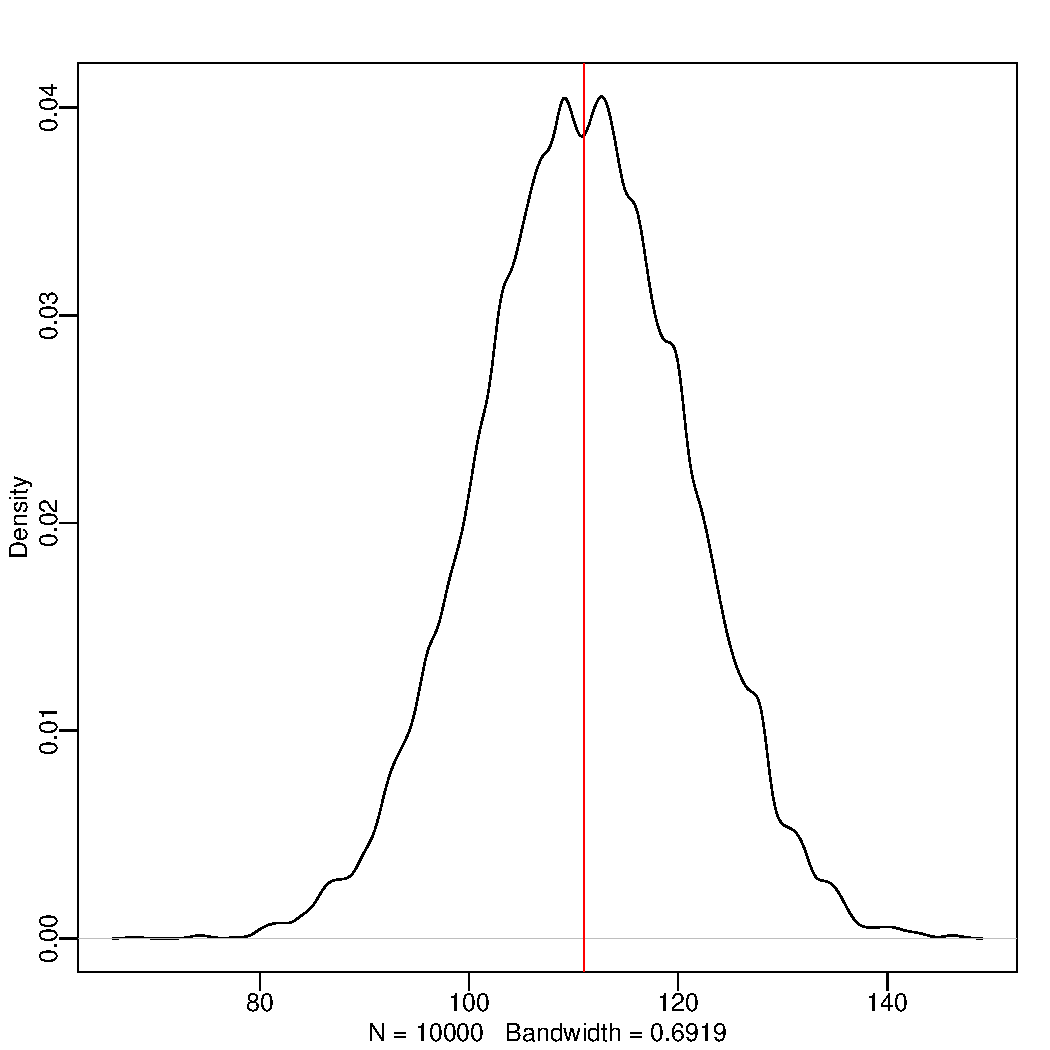
\includegraphics[width=\maxwidth]{figure/unnamed-chunk-19-1} 

\end{knitrout}

The peak of the distribution appears to be close to the true number of boys in the births (111 out of 200), so the distribution of predictions includes the actual observation as a central, likely outcome. Thus, it appears like the model fits the data well.

\begin{problem}{3H4}
\text{}\\
Now compare 10,000 counts of boys from 100 simulated first borns only to the number of boys in the first births, birth1. How does the model look in this light?
\end{problem}

\begin{knitrout}
\definecolor{shadecolor}{rgb}{0.969, 0.969, 0.969}\color{fgcolor}\begin{kframe}
\begin{alltt}
\hlstd{w} \hlkwb{<-} \hlkwd{rbinom}\hlstd{(}\hlnum{1e4}\hlstd{,} \hlkwc{size} \hlstd{=} \hlnum{100}\hlstd{,} \hlkwc{prob} \hlstd{= samples)}

\hlcom{#Number of boys in birth1}
\hlkwd{sum}\hlstd{(birth1)}
\end{alltt}
\begin{verbatim}
## [1] 51
\end{verbatim}
\begin{alltt}
\hlkwd{dens}\hlstd{(w)}
\hlkwd{abline}\hlstd{(}\hlkwc{v} \hlstd{=} \hlkwd{sum}\hlstd{(birth1),} \hlkwc{col} \hlstd{=} \hlstr{"red"}\hlstd{)}
\end{alltt}
\end{kframe}
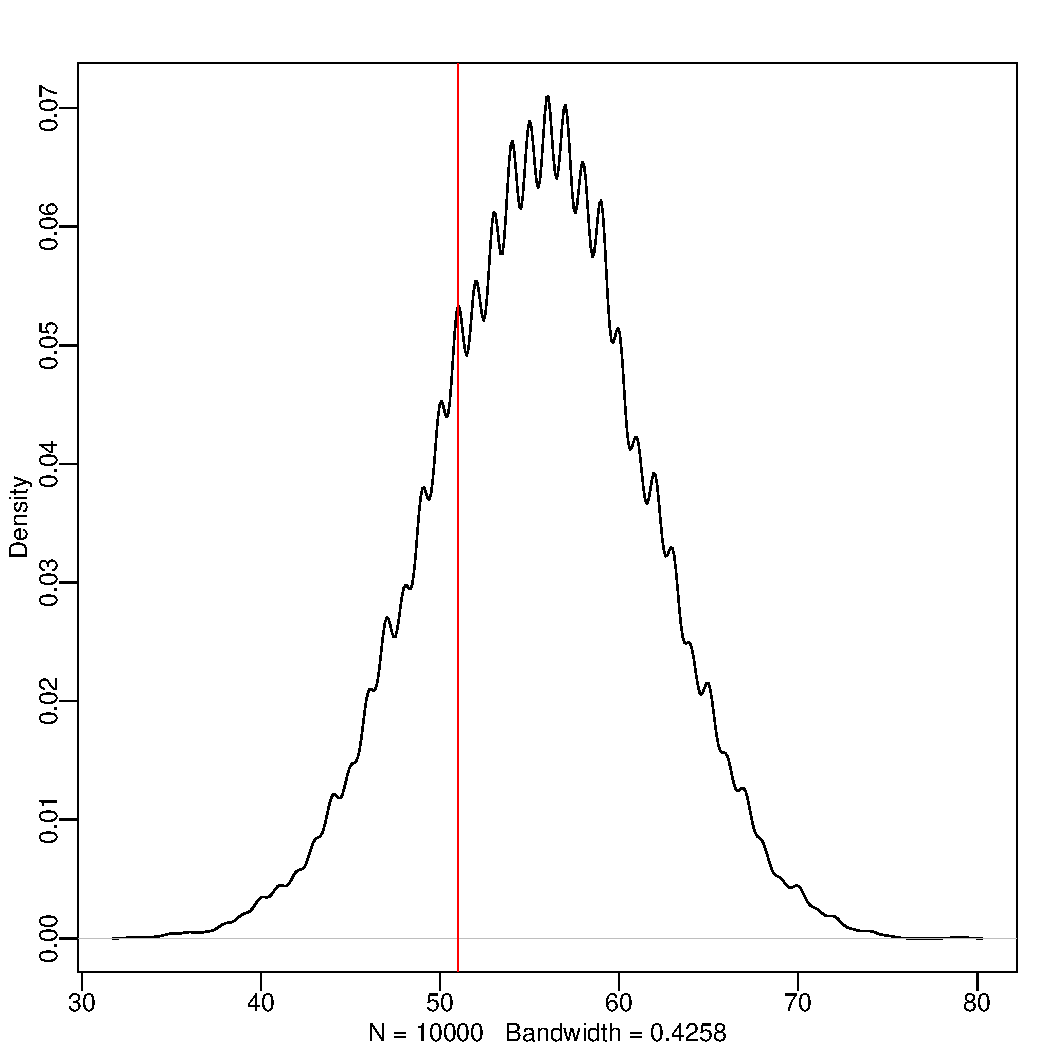
\includegraphics[width=\maxwidth]{figure/unnamed-chunk-20-1} 

\end{knitrout}

The model looks worse when comparing only to birth1. The peak of the distribution appears to be closer to 60, while there were 51 boys in birth1.

\begin{problem}{3H5}
\text{}\\
The model assumes that sex of first and second births are independent. To check this assumption, focus now on second births that followed female first borns. Compare 10,000 simulated counts of boys to only those second births that followed girls. To do this correctly, you need to count the number of first borns who were girls and simulate that many births, 10,000 times. Compare the count of boys in your simulations to the actual observed count of boys following girls. How does the model look in this light? Any guesses what is going on in the data?
\end{problem}

\begin{knitrout}
\definecolor{shadecolor}{rgb}{0.969, 0.969, 0.969}\color{fgcolor}\begin{kframe}
\begin{alltt}
\hlcom{#Number of first borns who were girls}
\hlstd{num_first_born_girls} \hlkwb{<-} \hlkwd{length}\hlstd{(birth1)} \hlopt{-} \hlkwd{sum}\hlstd{(birth1)}

\hlstd{w} \hlkwb{<-} \hlkwd{rbinom}\hlstd{(}\hlnum{1e4}\hlstd{,} \hlkwc{size} \hlstd{= num_first_born_girls,} \hlkwc{prob} \hlstd{= samples)}

\hlstd{boys_following_girls} \hlkwb{<-} \hlstd{birth2[birth1} \hlopt{==} \hlnum{0} \hlopt{&} \hlstd{birth2} \hlopt{==} \hlnum{1}\hlstd{]}

\hlcom{#Number of boys born after a girl}
\hlkwd{sum}\hlstd{(boys_following_girls)}
\end{alltt}
\begin{verbatim}
## [1] 39
\end{verbatim}
\begin{alltt}
\hlkwd{dens}\hlstd{(w)}
\hlkwd{abline}\hlstd{(}\hlkwc{v} \hlstd{=} \hlkwd{sum}\hlstd{(boys_following_girls),} \hlkwc{col} \hlstd{=} \hlstr{"red"}\hlstd{)}
\end{alltt}
\end{kframe}
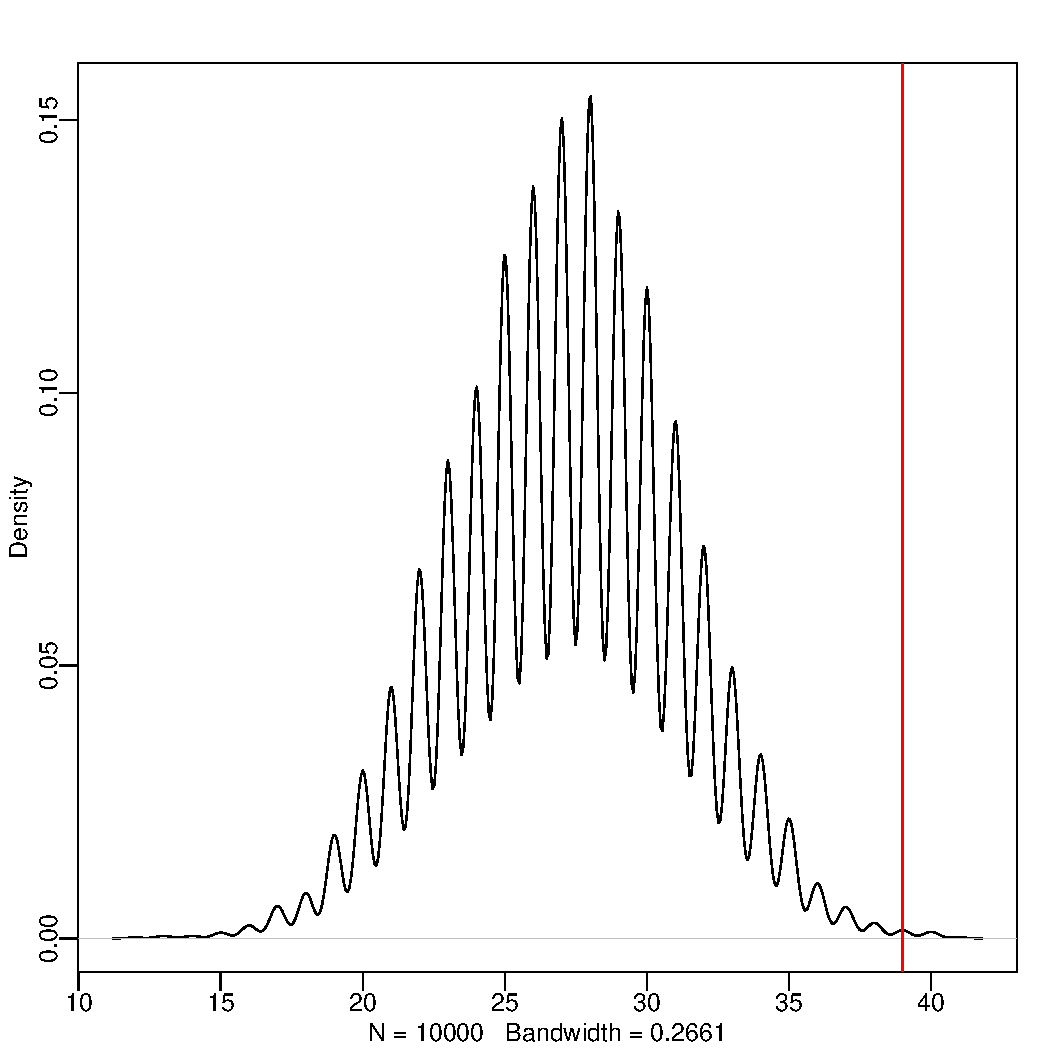
\includegraphics[width=\maxwidth]{figure/unnamed-chunk-21-1} 

\end{knitrout}

The model appears to fail spectacularly in this instance. The true number of boys born after girls is 39, yet the density value is miniscule for this number. It is possible that the model is assuming that the first and second births are independent, while they may not be in reality.

\end{document}
